\documentclass[1p]{elsarticle_modified}
%\bibliographystyle{elsarticle-num}

%\usepackage[colorlinks]{hyperref}
%\usepackage{abbrmath_seonhwa} %\Abb, \Ascr, \Acal ,\Abf, \Afrak
\usepackage{amsfonts}
\usepackage{amssymb}
\usepackage{amsmath}
\usepackage{amsthm}
\usepackage{scalefnt}
\usepackage{amsbsy}
\usepackage{kotex}
\usepackage{caption}
\usepackage{subfig}
\usepackage{color}
\usepackage{graphicx}
\usepackage{xcolor} %% white, black, red, green, blue, cyan, magenta, yellow
\usepackage{float}
\usepackage{setspace}
\usepackage{hyperref}

\usepackage{tikz}
\usetikzlibrary{arrows}

\usepackage{multirow}
\usepackage{array} % fixed length table
\usepackage{hhline}

%%%%%%%%%%%%%%%%%%%%%
\makeatletter
\renewcommand*\env@matrix[1][\arraystretch]{%
	\edef\arraystretch{#1}%
	\hskip -\arraycolsep
	\let\@ifnextchar\new@ifnextchar
	\array{*\c@MaxMatrixCols c}}
\makeatother %https://tex.stackexchange.com/questions/14071/how-can-i-increase-the-line-spacing-in-a-matrix
%%%%%%%%%%%%%%%

\usepackage[normalem]{ulem}

\newcommand{\msout}[1]{\ifmmode\text{\sout{\ensuremath{#1}}}\else\sout{#1}\fi}
%SOURCE: \msout is \stkout macro in https://tex.stackexchange.com/questions/20609/strikeout-in-math-mode

\newcommand{\cancel}[1]{
	\ifmmode
	{\color{red}\msout{#1}}
	\else
	{\color{red}\sout{#1}}
	\fi
}

\newcommand{\add}[1]{
	{\color{blue}\uwave{#1}}
}

\newcommand{\replace}[2]{
	\ifmmode
	{\color{red}\msout{#1}}{\color{blue}\uwave{#2}}
	\else
	{\color{red}\sout{#1}}{\color{blue}\uwave{#2}}
	\fi
}

\newcommand{\Sol}{\mathcal{S}} %segment
\newcommand{\D}{D} %diagram
\newcommand{\A}{\mathcal{A}} %arc


%%%%%%%%%%%%%%%%%%%%%%%%%%%%%5 test

\def\sl{\operatorname{\textup{SL}}(2,\Cbb)}
\def\psl{\operatorname{\textup{PSL}}(2,\Cbb)}
\def\quan{\mkern 1mu \triangleright \mkern 1mu}

\theoremstyle{definition}
\newtheorem{thm}{Theorem}[section]
\newtheorem{prop}[thm]{Proposition}
\newtheorem{lem}[thm]{Lemma}
\newtheorem{ques}[thm]{Question}
\newtheorem{cor}[thm]{Corollary}
\newtheorem{defn}[thm]{Definition}
\newtheorem{exam}[thm]{Example}
\newtheorem{rmk}[thm]{Remark}
\newtheorem{alg}[thm]{Algorithm}

\newcommand{\I}{\sqrt{-1}}
\begin{document}

%\begin{frontmatter}
%
%\title{Boundary parabolic representations of knots up to 8 crossings}
%
%%% Group authors per affiliation:
%\author{Yunhi Cho} 
%\address{Department of Mathematics, University of Seoul, Seoul, Korea}
%\ead{yhcho@uos.ac.kr}
%
%
%\author{Seonhwa Kim} %\fnref{s_kim}}
%\address{Center for Geometry and Physics, Institute for Basic Science, Pohang, 37673, Korea}
%\ead{ryeona17@ibs.re.kr}
%
%\author{Hyuk Kim}
%\address{Department of Mathematical Sciences, Seoul National University, Seoul 08826, Korea}
%\ead{hyukkim@snu.ac.kr}
%
%\author{Seokbeom Yoon}
%\address{Department of Mathematical Sciences, Seoul National University, Seoul, 08826,  Korea}
%\ead{sbyoon15@snu.ac.kr}
%
%\begin{abstract}
%We find all boundary parabolic representation of knots up to 8 crossings.
%
%\end{abstract}
%\begin{keyword}
%    \MSC[2010] 57M25 
%\end{keyword}
%
%\end{frontmatter}

%\linenumbers
%\tableofcontents
%
\newcommand\colored[1]{\textcolor{white}{\rule[-0.35ex]{0.8em}{1.4ex}}\kern-0.8em\color{red} #1}%
%\newcommand\colored[1]{\textcolor{white}{ #1}\kern-2.17ex	\textcolor{white}{ #1}\kern-1.81ex	\textcolor{white}{ #1}\kern-2.15ex\color{red}#1	}

{\Large $\underline{12n_{0175}~(K12n_{0175})}$}

\setlength{\tabcolsep}{10pt}
\renewcommand{\arraystretch}{1.6}
\vspace{1cm}\begin{tabular}{m{100pt}>{\centering\arraybackslash}m{274pt}}
\multirow{5}{120pt}{
	\centering
	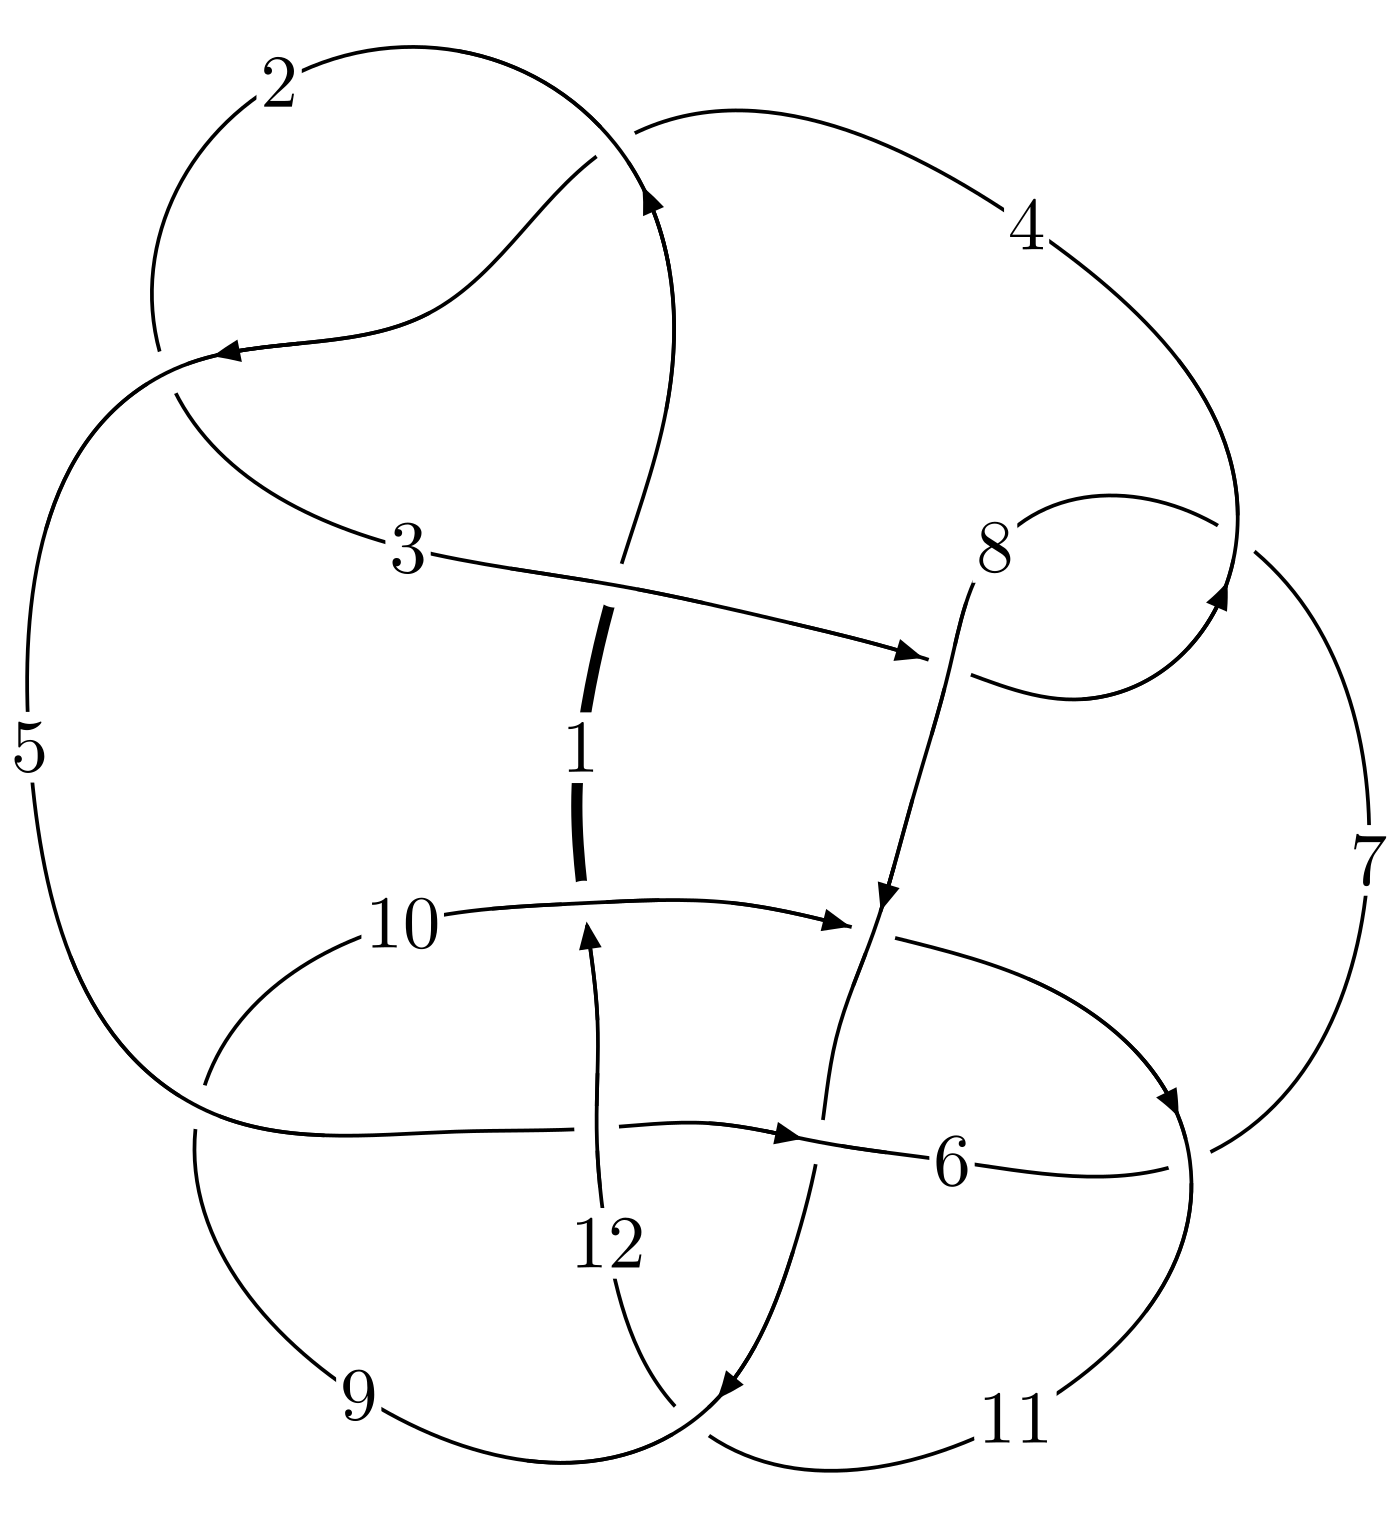
\includegraphics[width=112pt]{../../../GIT/diagram.site/Diagrams/png/2264_12n_0175.png}\\
\ \ \ A knot diagram\footnotemark}&
\allowdisplaybreaks
\textbf{Linearized knot diagam} \\
\cline{2-2}
 &
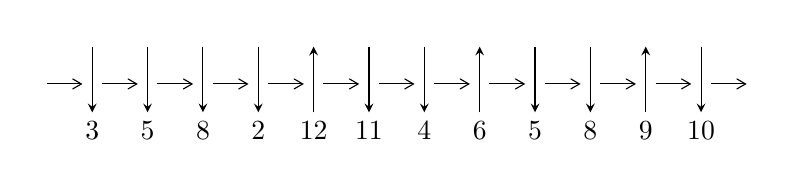
\begin{tikzpicture}[x=20pt, y=17pt]
	% nodes
	\node (C0) at (0, 0) {};
	\node (C1) at (1, 0) {};
	\node (C1U) at (1, +1) {};
	\node (C1D) at (1, -1) {3};

	\node (C2) at (2, 0) {};
	\node (C2U) at (2, +1) {};
	\node (C2D) at (2, -1) {5};

	\node (C3) at (3, 0) {};
	\node (C3U) at (3, +1) {};
	\node (C3D) at (3, -1) {8};

	\node (C4) at (4, 0) {};
	\node (C4U) at (4, +1) {};
	\node (C4D) at (4, -1) {2};

	\node (C5) at (5, 0) {};
	\node (C5U) at (5, +1) {};
	\node (C5D) at (5, -1) {12};

	\node (C6) at (6, 0) {};
	\node (C6U) at (6, +1) {};
	\node (C6D) at (6, -1) {11};

	\node (C7) at (7, 0) {};
	\node (C7U) at (7, +1) {};
	\node (C7D) at (7, -1) {4};

	\node (C8) at (8, 0) {};
	\node (C8U) at (8, +1) {};
	\node (C8D) at (8, -1) {6};

	\node (C9) at (9, 0) {};
	\node (C9U) at (9, +1) {};
	\node (C9D) at (9, -1) {5};

	\node (C10) at (10, 0) {};
	\node (C10U) at (10, +1) {};
	\node (C10D) at (10, -1) {8};

	\node (C11) at (11, 0) {};
	\node (C11U) at (11, +1) {};
	\node (C11D) at (11, -1) {9};

	\node (C12) at (12, 0) {};
	\node (C12U) at (12, +1) {};
	\node (C12D) at (12, -1) {10};
	\node (C13) at (13, 0) {};

	% arrows
	\draw[->,>={angle 60}]
	(C0) edge (C1) (C1) edge (C2) (C2) edge (C3) (C3) edge (C4) (C4) edge (C5) (C5) edge (C6) (C6) edge (C7) (C7) edge (C8) (C8) edge (C9) (C9) edge (C10) (C10) edge (C11) (C11) edge (C12) (C12) edge (C13) ;	\draw[->,>=stealth]
	(C1U) edge (C1D) (C2U) edge (C2D) (C3U) edge (C3D) (C4U) edge (C4D) (C5D) edge (C5U) (C6U) edge (C6D) (C7U) edge (C7D) (C8D) edge (C8U) (C9U) edge (C9D) (C10U) edge (C10D) (C11D) edge (C11U) (C12U) edge (C12D) ;
	\end{tikzpicture} \\
\hhline{~~} \\& 
\textbf{Solving Sequence} \\ \cline{2-2} 
 &
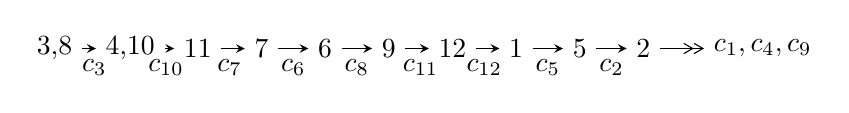
\begin{tikzpicture}[x=23pt, y=7pt]
	% node
	\node (A0) at (-1/8, 0) {3,8};
	\node (A1) at (17/16, 0) {4,10};
	\node (A2) at (17/8, 0) {11};
	\node (A3) at (25/8, 0) {7};
	\node (A4) at (33/8, 0) {6};
	\node (A5) at (41/8, 0) {9};
	\node (A6) at (49/8, 0) {12};
	\node (A7) at (57/8, 0) {1};
	\node (A8) at (65/8, 0) {5};
	\node (A9) at (73/8, 0) {2};
	\node (C1) at (1/2, -1) {$c_{3}$};
	\node (C2) at (13/8, -1) {$c_{10}$};
	\node (C3) at (21/8, -1) {$c_{7}$};
	\node (C4) at (29/8, -1) {$c_{6}$};
	\node (C5) at (37/8, -1) {$c_{8}$};
	\node (C6) at (45/8, -1) {$c_{11}$};
	\node (C7) at (53/8, -1) {$c_{12}$};
	\node (C8) at (61/8, -1) {$c_{5}$};
	\node (C9) at (69/8, -1) {$c_{2}$};
	\node (A10) at (11, 0) {$c_{1},c_{4},c_{9}$};

	% edge
	\draw[->,>=stealth]	
	(A0) edge (A1) (A1) edge (A2) (A2) edge (A3) (A3) edge (A4) (A4) edge (A5) (A5) edge (A6) (A6) edge (A7) (A7) edge (A8) (A8) edge (A9) ;
	\draw[->>,>={angle 60}]	
	(A9) edge (A10);
\end{tikzpicture} \\ 

\end{tabular} \\

\footnotetext{
The image of knot diagram is generated by the software ``\textbf{Draw programme}" developed by Andrew Bartholomew(\url{http://www.layer8.co.uk/maths/draw/index.htm\#Running-draw}), where we modified some parts for our purpose(\url{https://github.com/CATsTAILs/LinksPainter}).
}\phantom \\ \newline 
\centering \textbf{Ideals for irreducible components\footnotemark of $X_{\text{par}}$} 
 
\begin{align*}
I^u_{1}&=\langle 
-1.04267\times10^{26} u^{13}-2.24065\times10^{27} u^{12}+\cdots+1.09231\times10^{29} b+2.46093\times10^{28},\\
\phantom{I^u_{1}}&\phantom{= \langle  }-1.28732\times10^{26} u^{13}-2.92904\times10^{27} u^{12}+\cdots+2.18462\times10^{29} a-1.14504\times10^{29},\\
\phantom{I^u_{1}}&\phantom{= \langle  }u^{14}+21 u^{13}+\cdots+544 u+256\rangle \\
I^u_{2}&=\langle 
-102 u^8-440 u^7-440 u^6-655 u^5+u^4-240 u^3+269 u^2+59 b-180 u+261,\\
\phantom{I^u_{2}}&\phantom{= \langle  }-15 u^8-30 u^7+88 u^6+72 u^5+283 u^4+107 u^3+253 u^2+59 a+36 u+172,\\
\phantom{I^u_{2}}&\phantom{= \langle  }u^9+5 u^8+8 u^7+13 u^6+10 u^5+11 u^4+5 u^3+6 u^2+u+1\rangle \\
I^u_{3}&=\langle 
-2 u^5 a+10 u^4 a-2 u^5-30 u^3 a+13 u^4+33 u^2 a-45 u^3-14 a u+78 u^2+6 b+4 a-62 u+28,\\
\phantom{I^u_{3}}&\phantom{= \langle  }18 u^5 a+39 u^5+\cdots+16 a-220,\;u^6-7 u^5+26 u^4-51 u^3+52 u^2-28 u+8\rangle \\
I^u_{4}&=\langle 
2 u^2 b+b^2- b u+4 u^2+4 b-2 u+7,\;u^2+a- u+2,\;u^3- u^2+2 u-1\rangle \\
\\
I^v_{1}&=\langle 
a,\;- v^3-7 v^2+4 b-12 v-1,\;v^4+7 v^3+16 v^2+13 v+4\rangle \\
I^v_{2}&=\langle 
a,\;- v^2 b+b^2+2 b v- v^2+b+2 v+1,\;v^3-3 v^2+2 v-1\rangle \\
\end{align*}
\raggedright * 6 irreducible components of $\dim_{\mathbb{C}}=0$, with total 51 representations.\\
\footnotetext{All coefficients of polynomials are rational numbers. But the coefficients are sometimes approximated in decimal forms when there is not enough margin.}
\newpage
\renewcommand{\arraystretch}{1}
\centering \section*{I. $I^u_{1}= \langle -1.04\times10^{26} u^{13}-2.24\times10^{27} u^{12}+\cdots+1.09\times10^{29} b+2.46\times10^{28},\;-1.29\times10^{26} u^{13}-2.93\times10^{27} u^{12}+\cdots+2.18\times10^{29} a-1.15\times10^{29},\;u^{14}+21 u^{13}+\cdots+544 u+256 \rangle$}
\flushleft \textbf{(i) Arc colorings}\\
\begin{tabular}{m{7pt} m{180pt} m{7pt} m{180pt} }
\flushright $a_{3}=$&$\begin{pmatrix}1\\0\end{pmatrix}$ \\
\flushright $a_{8}=$&$\begin{pmatrix}0\\u\end{pmatrix}$ \\
\flushright $a_{4}=$&$\begin{pmatrix}1\\u^2\end{pmatrix}$ \\
\flushright $a_{10}=$&$\begin{pmatrix}0.000589262 u^{13}+0.0134075 u^{12}+\cdots-0.805195 u+0.524136\\0.000954555 u^{13}+0.0205129 u^{12}+\cdots+0.318887 u-0.225296\end{pmatrix}$ \\
\flushright $a_{11}=$&$\begin{pmatrix}0.000589262 u^{13}+0.0134075 u^{12}+\cdots-0.805195 u+0.524136\\0.000671621 u^{13}+0.0148039 u^{12}+\cdots-0.393936 u-0.489753\end{pmatrix}$ \\
\flushright $a_{7}=$&$\begin{pmatrix}u\\u^3+u\end{pmatrix}$ \\
\flushright $a_{6}=$&$\begin{pmatrix}0.00121747 u^{13}+0.0251618 u^{12}+\cdots+2.10350 u+0.0491900\\0.000115085 u^{13}+0.00299760 u^{12}+\cdots+0.828767 u-0.0553136\end{pmatrix}$ \\
\flushright $a_{9}=$&$\begin{pmatrix}0.00122256 u^{13}+0.0260104 u^{12}+\cdots+0.0388506 u+0.499449\\0.000709347 u^{13}+0.0153553 u^{12}+\cdots+0.361561 u-0.145546\end{pmatrix}$ \\
\flushright $a_{12}=$&$\begin{pmatrix}0.000261393 u^{13}+0.00718595 u^{12}+\cdots-1.58109 u+0.503456\\0.00106954 u^{13}+0.0235741 u^{12}+\cdots-0.362940 u-0.280603\end{pmatrix}$ \\
\flushright $a_{1}=$&$\begin{pmatrix}0.000424271 u^{13}+0.00989082 u^{12}+\cdots-0.674232 u+0.474041\\0.0000149496 u^{13}+0.00111721 u^{12}+\cdots-0.559577 u-0.359209\end{pmatrix}$ \\
\flushright $a_{5}=$&$\begin{pmatrix}-0.000409321 u^{13}-0.00877361 u^{12}+\cdots+0.114654 u-0.833250\\0.0000359381 u^{13}+0.00108264 u^{12}+\cdots-0.358027 u-0.313673\end{pmatrix}$ \\
\flushright $a_{2}=$&$\begin{pmatrix}0.000409321 u^{13}+0.00877361 u^{12}+\cdots-0.114654 u+0.833250\\0.0000149496 u^{13}+0.00111721 u^{12}+\cdots-0.559577 u-0.359209\end{pmatrix}$\\&\end{tabular}
\flushleft \textbf{(ii) Obstruction class $= -1$}\\~\\
\flushleft \textbf{(iii) Cusp Shapes $= -0.00674689 u^{13}-0.136707 u^{12}+\cdots-11.6248 u-11.8608$}\\~\\
\newpage\renewcommand{\arraystretch}{1}
\flushleft \textbf{(iv) u-Polynomials at the component}\newline \\
\begin{tabular}{m{50pt}|m{274pt}}
Crossings & \hspace{64pt}u-Polynomials at each crossing \\
\hline $$\begin{aligned}c_{1}\end{aligned}$$&$\begin{aligned}
&u^{14}+54 u^{13}+\cdots-7647 u+256
\end{aligned}$\\
\hline $$\begin{aligned}c_{2},c_{4}\end{aligned}$$&$\begin{aligned}
&u^{14}-16 u^{13}+\cdots+31 u-16
\end{aligned}$\\
\hline $$\begin{aligned}c_{3},c_{7}\end{aligned}$$&$\begin{aligned}
&u^{14}+21 u^{13}+\cdots+544 u+256
\end{aligned}$\\
\hline $$\begin{aligned}c_{5},c_{8}\end{aligned}$$&$\begin{aligned}
&u^{14}+2 u^{13}+\cdots+4 u+1
\end{aligned}$\\
\hline $$\begin{aligned}c_{6},c_{9}\end{aligned}$$&$\begin{aligned}
&u^{14}-11 u^{13}+\cdots+9 u-9
\end{aligned}$\\
\hline $$\begin{aligned}c_{10},c_{12}\end{aligned}$$&$\begin{aligned}
&u^{14}+27 u^{13}+\cdots+157 u-1
\end{aligned}$\\
\hline $$\begin{aligned}c_{11}\end{aligned}$$&$\begin{aligned}
&u^{14}+22 u^{13}+\cdots+88 u+4
\end{aligned}$\\
\hline
\end{tabular}\\~\\
\newpage\renewcommand{\arraystretch}{1}
\flushleft \textbf{(v) Riley Polynomials at the component}\newline \\
\begin{tabular}{m{50pt}|m{274pt}}
Crossings & \hspace{64pt}Riley Polynomials at each crossing \\
\hline $$\begin{aligned}c_{1}\end{aligned}$$&$\begin{aligned}
&y^{14}-910 y^{13}+\cdots-40412737 y+65536
\end{aligned}$\\
\hline $$\begin{aligned}c_{2},c_{4}\end{aligned}$$&$\begin{aligned}
&y^{14}-54 y^{13}+\cdots+7647 y+256
\end{aligned}$\\
\hline $$\begin{aligned}c_{3},c_{7}\end{aligned}$$&$\begin{aligned}
&y^{14}-177 y^{13}+\cdots-226304 y+65536
\end{aligned}$\\
\hline $$\begin{aligned}c_{5},c_{8}\end{aligned}$$&$\begin{aligned}
&y^{14}-2 y^{13}+\cdots-6 y+1
\end{aligned}$\\
\hline $$\begin{aligned}c_{6},c_{9}\end{aligned}$$&$\begin{aligned}
&y^{14}-61 y^{13}+\cdots-927 y+81
\end{aligned}$\\
\hline $$\begin{aligned}c_{10},c_{12}\end{aligned}$$&$\begin{aligned}
&y^{14}-413 y^{13}+\cdots-22155 y+1
\end{aligned}$\\
\hline $$\begin{aligned}c_{11}\end{aligned}$$&$\begin{aligned}
&y^{14}-64 y^{13}+\cdots-2456 y+16
\end{aligned}$\\
\hline
\end{tabular}\\~\\
\newpage\flushleft \textbf{(vi) Complex Volumes and Cusp Shapes}
$$\begin{array}{c|c|c}  
\text{Solutions to }I^u_{1}& \I (\text{vol} + \sqrt{-1}CS) & \text{Cusp shape}\\
 \hline 
\begin{aligned}
u &= -0.126413 + 1.064170 I \\
a &= \phantom{-}0.0178207 - 0.1327570 I \\
b &= \phantom{-}0.073229 + 0.409880 I\end{aligned}
 & \phantom{-}2.38888 + 2.31349 I & \phantom{-}1.040974 + 0.185703 I \\ \hline\begin{aligned}
u &= -0.126413 - 1.064170 I \\
a &= \phantom{-}0.0178207 + 0.1327570 I \\
b &= \phantom{-}0.073229 - 0.409880 I\end{aligned}
 & \phantom{-}2.38888 - 2.31349 I & \phantom{-}1.040974 - 0.185703 I \\ \hline\begin{aligned}
u &= \phantom{-}0.594510 + 0.411375 I \\
a &= -0.944868 + 0.799301 I \\
b &= -0.88821 + 1.42199 I\end{aligned}
 & -3.64308 + 0.88750 I & -15.9778 + 0.0604 I \\ \hline\begin{aligned}
u &= \phantom{-}0.594510 - 0.411375 I \\
a &= -0.944868 - 0.799301 I \\
b &= -0.88821 - 1.42199 I\end{aligned}
 & -3.64308 - 0.88750 I & -15.9778 - 0.0604 I \\ \hline\begin{aligned}
u &= \phantom{-}1.40610 + 0.22467 I \\
a &= \phantom{-}0.307958 + 1.309810 I \\
b &= \phantom{-}0.030088 + 0.287966 I\end{aligned}
 & \phantom{-}0.10775 - 7.50729 I & -7.28452 + 4.95143 I \\ \hline\begin{aligned}
u &= \phantom{-}1.40610 - 0.22467 I \\
a &= \phantom{-}0.307958 - 1.309810 I \\
b &= \phantom{-}0.030088 - 0.287966 I\end{aligned}
 & \phantom{-}0.10775 + 7.50729 I & -7.28452 - 4.95143 I \\ \hline\begin{aligned}
u &= -0.560428\phantom{ +0.000000I} \\
a &= -0.0120122\phantom{ +0.000000I} \\
b &= -0.522964\phantom{ +0.000000I}\end{aligned}
 & -1.12206\phantom{ +0.000000I} & -9.20330\phantom{ +0.000000I} \\ \hline\begin{aligned}
u &= -0.345517 + 0.363205 I \\
a &= \phantom{-}1.121570 + 0.274743 I \\
b &= -0.330774 + 0.391733 I\end{aligned}
 & -0.921235 + 1.059300 I & -5.51258 - 4.57245 I \\ \hline\begin{aligned}
u &= -0.345517 - 0.363205 I \\
a &= \phantom{-}1.121570 - 0.274743 I \\
b &= -0.330774 - 0.391733 I\end{aligned}
 & -0.921235 - 1.059300 I & -5.51258 + 4.57245 I \\ \hline\begin{aligned}
u &= -1.80958 + 2.11291 I \\
a &= -1.248730 - 0.134703 I \\
b &= -2.16984 + 0.05278 I\end{aligned}
 & \phantom{-}19.0076 + 14.9612 I & -6.21836 - 5.88234 I\\
 \hline 
 \end{array}$$\newpage$$\begin{array}{c|c|c}  
\text{Solutions to }I^u_{1}& \I (\text{vol} + \sqrt{-1}CS) & \text{Cusp shape}\\
 \hline 
\begin{aligned}
u &= -1.80958 - 2.11291 I \\
a &= -1.248730 + 0.134703 I \\
b &= -2.16984 - 0.05278 I\end{aligned}
 & \phantom{-}19.0076 - 14.9612 I & -6.21836 + 5.88234 I \\ \hline\begin{aligned}
u &= -3.79852 + 1.13400 I \\
a &= \phantom{-}1.41552 + 0.05510 I \\
b &= \phantom{-}2.07852 + 0.02544 I\end{aligned}
 & -18.1348 - 0.1387 I & -2.93027 + 5.79154 I \\ \hline\begin{aligned}
u &= -3.79852 - 1.13400 I \\
a &= \phantom{-}1.41552 - 0.05510 I \\
b &= \phantom{-}2.07852 - 0.02544 I\end{aligned}
 & -18.1348 + 0.1387 I & -2.93027 - 5.79154 I \\ \hline\begin{aligned}
u &= -12.2807\phantom{ +0.000000I} \\
a &= \phantom{-}1.54847\phantom{ +0.000000I} \\
b &= \phantom{-}2.18693\phantom{ +0.000000I}\end{aligned}
 & -17.8723\phantom{ +0.000000I} & \phantom{-0.000000 } 0\\
 \hline 
 \end{array}$$\newpage\newpage\renewcommand{\arraystretch}{1}
\centering \section*{II. $I^u_{2}= \langle -102 u^8-440 u^7+\cdots+59 b+261,\;-15 u^8-30 u^7+\cdots+59 a+172,\;u^9+5 u^8+\cdots+u+1 \rangle$}
\flushleft \textbf{(i) Arc colorings}\\
\begin{tabular}{m{7pt} m{180pt} m{7pt} m{180pt} }
\flushright $a_{3}=$&$\begin{pmatrix}1\\0\end{pmatrix}$ \\
\flushright $a_{8}=$&$\begin{pmatrix}0\\u\end{pmatrix}$ \\
\flushright $a_{4}=$&$\begin{pmatrix}1\\u^2\end{pmatrix}$ \\
\flushright $a_{10}=$&$\begin{pmatrix}0.254237 u^{8}+0.508475 u^{7}+\cdots-0.610169 u-2.91525\\1.72881 u^{8}+7.45763 u^{7}+\cdots+3.05085 u-4.42373\end{pmatrix}$ \\
\flushright $a_{11}=$&$\begin{pmatrix}0.254237 u^{8}+0.508475 u^{7}+\cdots-0.610169 u-2.91525\\2.01695 u^{8}+9.03390 u^{7}+\cdots+3.55932 u-3.66102\end{pmatrix}$ \\
\flushright $a_{7}=$&$\begin{pmatrix}u\\u^3+u\end{pmatrix}$ \\
\flushright $a_{6}=$&$\begin{pmatrix}-1.08475 u^{8}-6.16949 u^{7}+\cdots-4.79661 u-2.69492\\-0.593220 u^{8}-4.18644 u^{7}+\cdots-3.57627 u-4.86441\end{pmatrix}$ \\
\flushright $a_{9}=$&$\begin{pmatrix}0.491525 u^{8}+1.98305 u^{7}+\cdots+1.22034 u-2.16949\\2.38983 u^{8}+10.7797 u^{7}+\cdots+5.86441 u-3.20339\end{pmatrix}$ \\
\flushright $a_{12}=$&$\begin{pmatrix}-1.23729 u^{8}-6.47458 u^{7}+\cdots-7.83051 u-1.74576\\-2.74576 u^{8}-14.4915 u^{7}+\cdots-13.6102 u-4.91525\end{pmatrix}$ \\
\flushright $a_{1}=$&$\begin{pmatrix}0.491525 u^{8}+1.98305 u^{7}+\cdots-0.779661 u-1.16949\\0.0677966 u^{8}+0.135593 u^{7}+\cdots-0.762712 u-1.64407\end{pmatrix}$ \\
\flushright $a_{5}=$&$\begin{pmatrix}0.423729 u^{8}+1.84746 u^{7}+\cdots-0.0169492 u+0.474576\\-0.254237 u^{8}-0.508475 u^{7}+\cdots+0.610169 u+1.91525\end{pmatrix}$ \\
\flushright $a_{2}=$&$\begin{pmatrix}0.423729 u^{8}+1.84746 u^{7}+\cdots-0.0169492 u+0.474576\\0.0677966 u^{8}+0.135593 u^{7}+\cdots-0.762712 u-1.64407\end{pmatrix}$\\&\end{tabular}
\flushleft \textbf{(ii) Obstruction class $= 1$}\\~\\
\flushleft \textbf{(iii) Cusp Shapes $= \frac{142}{59} u^8+\frac{756}{59} u^7+\frac{1287}{59} u^6+\frac{1997}{59} u^5+\frac{2096}{59} u^4+\frac{1528}{59} u^3+\frac{1554}{59} u^2+\frac{792}{59} u+\frac{480}{59}$}\\~\\
\newpage\renewcommand{\arraystretch}{1}
\flushleft \textbf{(iv) u-Polynomials at the component}\newline \\
\begin{tabular}{m{50pt}|m{274pt}}
Crossings & \hspace{64pt}u-Polynomials at each crossing \\
\hline $$\begin{aligned}c_{1}\end{aligned}$$&$\begin{aligned}
&u^9-10 u^8+29 u^7-39 u^6+26 u^5-15 u^4+19 u^3-8 u^2-3 u-1
\end{aligned}$\\
\hline $$\begin{aligned}c_{2}\end{aligned}$$&$\begin{aligned}
&u^9+4 u^8+3 u^7-5 u^6-10 u^5-5 u^4+3 u^3+6 u^2+3 u+1
\end{aligned}$\\
\hline $$\begin{aligned}c_{3}\end{aligned}$$&$\begin{aligned}
&u^9+5 u^8+8 u^7+13 u^6+10 u^5+11 u^4+5 u^3+6 u^2+u+1
\end{aligned}$\\
\hline $$\begin{aligned}c_{4}\end{aligned}$$&$\begin{aligned}
&u^9-4 u^8+3 u^7+5 u^6-10 u^5+5 u^4+3 u^3-6 u^2+3 u-1
\end{aligned}$\\
\hline $$\begin{aligned}c_{5},c_{8}\end{aligned}$$&$\begin{aligned}
&u^9-3 u^8+5 u^7-4 u^6+2 u^5-2 u^4+4 u^3-3 u^2+1
\end{aligned}$\\
\hline $$\begin{aligned}c_{6},c_{9}\end{aligned}$$&$\begin{aligned}
&u^9-3 u^7+4 u^6-2 u^5+2 u^4-4 u^3+5 u^2-3 u+1
\end{aligned}$\\
\hline $$\begin{aligned}c_{7}\end{aligned}$$&$\begin{aligned}
&u^9-5 u^8+8 u^7-13 u^6+10 u^5-11 u^4+5 u^3-6 u^2+u-1
\end{aligned}$\\
\hline $$\begin{aligned}c_{10},c_{12}\end{aligned}$$&$\begin{aligned}
&u^9+6 u^8+5 u^7+12 u^6+6 u^5+10 u^4+5 u^2- u+1
\end{aligned}$\\
\hline $$\begin{aligned}c_{11}\end{aligned}$$&$\begin{aligned}
&u^9-3 u^8-7 u^7+61 u^6-171 u^5+279 u^4-297 u^3+212 u^2-97 u+23
\end{aligned}$\\
\hline
\end{tabular}\\~\\
\newpage\renewcommand{\arraystretch}{1}
\flushleft \textbf{(v) Riley Polynomials at the component}\newline \\
\begin{tabular}{m{50pt}|m{274pt}}
Crossings & \hspace{64pt}Riley Polynomials at each crossing \\
\hline $$\begin{aligned}c_{1}\end{aligned}$$&$\begin{aligned}
&y^9-42 y^8+\cdots-7 y-1
\end{aligned}$\\
\hline $$\begin{aligned}c_{2},c_{4}\end{aligned}$$&$\begin{aligned}
&y^9-10 y^8+29 y^7-39 y^6+26 y^5-15 y^4+19 y^3-8 y^2-3 y-1
\end{aligned}$\\
\hline $$\begin{aligned}c_{3},c_{7}\end{aligned}$$&$\begin{aligned}
&y^9-9 y^8-46 y^7-109 y^6-164 y^5-171 y^4-113 y^3-48 y^2-11 y-1
\end{aligned}$\\
\hline $$\begin{aligned}c_{5},c_{8}\end{aligned}$$&$\begin{aligned}
&y^9+y^8+5 y^7+10 y^5-6 y^4+12 y^3-5 y^2+6 y-1
\end{aligned}$\\
\hline $$\begin{aligned}c_{6},c_{9}\end{aligned}$$&$\begin{aligned}
&y^9-6 y^8+5 y^7-12 y^6+6 y^5-10 y^4-5 y^2- y-1
\end{aligned}$\\
\hline $$\begin{aligned}c_{10},c_{12}\end{aligned}$$&$\begin{aligned}
&y^9-26 y^8+\cdots-9 y-1
\end{aligned}$\\
\hline $$\begin{aligned}c_{11}\end{aligned}$$&$\begin{aligned}
&y^9-23 y^8+\cdots-343 y-529
\end{aligned}$\\
\hline
\end{tabular}\\~\\
\newpage\flushleft \textbf{(vi) Complex Volumes and Cusp Shapes}
$$\begin{array}{c|c|c}  
\text{Solutions to }I^u_{2}& \I (\text{vol} + \sqrt{-1}CS) & \text{Cusp shape}\\
 \hline 
\begin{aligned}
u &= -0.699225 + 0.881171 I \\
a &= \phantom{-}0.153901 - 0.439956 I \\
b &= -0.480829 - 0.332872 I\end{aligned}
 & -1.28188 + 7.91801 I & -11.0500 - 9.5481 I \\ \hline\begin{aligned}
u &= -0.699225 - 0.881171 I \\
a &= \phantom{-}0.153901 + 0.439956 I \\
b &= -0.480829 + 0.332872 I\end{aligned}
 & -1.28188 - 7.91801 I & -11.0500 + 9.5481 I \\ \hline\begin{aligned}
u &= -0.293070 + 1.131440 I \\
a &= -0.518996 + 0.755920 I \\
b &= -0.365565 - 0.116422 I\end{aligned}
 & \phantom{-}1.91580 - 3.10870 I & -3.25080 + 5.79361 I \\ \hline\begin{aligned}
u &= -0.293070 - 1.131440 I \\
a &= -0.518996 - 0.755920 I \\
b &= -0.365565 + 0.116422 I\end{aligned}
 & \phantom{-}1.91580 + 3.10870 I & -3.25080 - 5.79361 I \\ \hline\begin{aligned}
u &= \phantom{-}0.355075 + 0.694524 I \\
a &= -0.776460 - 0.463249 I \\
b &= \phantom{-}0.258201 - 0.760917 I\end{aligned}
 & \phantom{-}1.44595 - 4.09337 I & -1.10458 + 4.89395 I \\ \hline\begin{aligned}
u &= \phantom{-}0.355075 - 0.694524 I \\
a &= -0.776460 + 0.463249 I \\
b &= \phantom{-}0.258201 + 0.760917 I\end{aligned}
 & \phantom{-}1.44595 + 4.09337 I & -1.10458 - 4.89395 I \\ \hline\begin{aligned}
u &= -0.046807 + 0.509508 I \\
a &= -2.11030 - 0.01768 I \\
b &= -3.48539 + 1.47690 I\end{aligned}
 & -1.03199 - 3.67986 I & \phantom{-}3.16209 + 3.89016 I \\ \hline\begin{aligned}
u &= -0.046807 - 0.509508 I \\
a &= -2.11030 + 0.01768 I \\
b &= -3.48539 - 1.47690 I\end{aligned}
 & -1.03199 + 3.67986 I & \phantom{-}3.16209 - 3.89016 I \\ \hline\begin{aligned}
u &= -3.63195\phantom{ +0.000000I} \\
a &= \phantom{-}1.50371\phantom{ +0.000000I} \\
b &= \phantom{-}2.14716\phantom{ +0.000000I}\end{aligned}
 & -18.5451\phantom{ +0.000000I} & -22.5130\phantom{ +0.000000I}\\
 \hline 
 \end{array}$$\newpage\newpage\renewcommand{\arraystretch}{1}
\centering \section*{III. $I^u_{3}= \langle -2 u^5 a-2 u^5+\cdots+4 a+28,\;18 u^5 a+39 u^5+\cdots+16 a-220,\;u^6-7 u^5+26 u^4-51 u^3+52 u^2-28 u+8 \rangle$}
\flushleft \textbf{(i) Arc colorings}\\
\begin{tabular}{m{7pt} m{180pt} m{7pt} m{180pt} }
\flushright $a_{3}=$&$\begin{pmatrix}1\\0\end{pmatrix}$ \\
\flushright $a_{8}=$&$\begin{pmatrix}0\\u\end{pmatrix}$ \\
\flushright $a_{4}=$&$\begin{pmatrix}1\\u^2\end{pmatrix}$ \\
\flushright $a_{10}=$&$\begin{pmatrix}a\\\frac{1}{3} u^5 a+\frac{1}{3} u^5+\cdots-\frac{2}{3} a-\frac{14}{3}\end{pmatrix}$ \\
\flushright $a_{11}=$&$\begin{pmatrix}a\\\frac{1}{3} u^5 a+\frac{1}{3} u^5+\cdots-\frac{2}{3} a-\frac{14}{3}\end{pmatrix}$ \\
\flushright $a_{7}=$&$\begin{pmatrix}u\\u^3+u\end{pmatrix}$ \\
\flushright $a_{6}=$&$\begin{pmatrix}\frac{1}{12} u^5 a-\frac{1}{3} u^5+\cdots-3 a+\frac{17}{6}\\\frac{1}{2} u^5 a-\frac{17}{12} u^5+\cdots-\frac{10}{3} a+3\end{pmatrix}$ \\
\flushright $a_{9}=$&$\begin{pmatrix}\frac{1}{6} u^5 a+\frac{1}{12} u^5+\cdots+\frac{2}{3} a-\frac{5}{2}\\\frac{7}{6} u^5 a+\frac{7}{12} u^5+\cdots-\frac{14}{3} a-\frac{19}{3}\end{pmatrix}$ \\
\flushright $a_{12}=$&$\begin{pmatrix}-\frac{1}{8} u^5+\frac{7}{8} u^4+\cdots-\frac{13}{2} u+\frac{7}{2}\\\frac{1}{6} u^5 a-\frac{19}{12} u^5+\cdots-\frac{8}{3} a+\frac{20}{3}\end{pmatrix}$ \\
\flushright $a_{1}=$&$\begin{pmatrix}\frac{19}{24} u^5-\frac{35}{8} u^4+\cdots+\frac{35}{3} u-3\\\frac{2}{3} u^5-\frac{11}{3} u^4+\cdots+\frac{32}{3} u-\frac{11}{3}\end{pmatrix}$ \\
\flushright $a_{5}=$&$\begin{pmatrix}-\frac{1}{8} u^5+\frac{17}{24} u^4+\cdots- u-\frac{2}{3}\\\frac{1}{2} u^5-\frac{17}{6} u^4+\cdots+7 u-\frac{7}{3}\end{pmatrix}$ \\
\flushright $a_{2}=$&$\begin{pmatrix}\frac{1}{8} u^5-\frac{17}{24} u^4+\cdots+u+\frac{2}{3}\\\frac{2}{3} u^5-\frac{11}{3} u^4+\cdots+\frac{32}{3} u-\frac{11}{3}\end{pmatrix}$\\&\end{tabular}
\flushleft \textbf{(ii) Obstruction class $= -1$}\\~\\
\flushleft \textbf{(iii) Cusp Shapes $= \frac{17}{12} u^5-\frac{85}{12} u^4+21 u^3-\frac{85}{4} u^2+\frac{25}{6} u-\frac{19}{3}$}\\~\\
\newpage\renewcommand{\arraystretch}{1}
\flushleft \textbf{(iv) u-Polynomials at the component}\newline \\
\begin{tabular}{m{50pt}|m{274pt}}
Crossings & \hspace{64pt}u-Polynomials at each crossing \\
\hline $$\begin{aligned}c_{1}\end{aligned}$$&$\begin{aligned}
&(u^6+4 u^5+24 u^4+11 u^3+42 u^2-11 u+1)^2
\end{aligned}$\\
\hline $$\begin{aligned}c_{2},c_{4}\end{aligned}$$&$\begin{aligned}
&(u^6-2 u^5+3 u^3+6 u^2- u+1)^2
\end{aligned}$\\
\hline $$\begin{aligned}c_{3},c_{7}\end{aligned}$$&$\begin{aligned}
&(u^6-7 u^5+26 u^4-51 u^3+52 u^2-28 u+8)^2
\end{aligned}$\\
\hline $$\begin{aligned}c_{5},c_{8}\end{aligned}$$&$\begin{aligned}
&u^{12}+2 u^{11}+\cdots+15 u+9
\end{aligned}$\\
\hline $$\begin{aligned}c_{6},c_{9}\end{aligned}$$&$\begin{aligned}
&u^{12}-6 u^{11}+\cdots-1017 u+603
\end{aligned}$\\
\hline $$\begin{aligned}c_{10},c_{12}\end{aligned}$$&$\begin{aligned}
&u^{12}- u^{11}+\cdots-942 u+423
\end{aligned}$\\
\hline $$\begin{aligned}c_{11}\end{aligned}$$&$\begin{aligned}
&(u^6- u^5+5 u^3-4 u+8)^2
\end{aligned}$\\
\hline
\end{tabular}\\~\\
\newpage\renewcommand{\arraystretch}{1}
\flushleft \textbf{(v) Riley Polynomials at the component}\newline \\
\begin{tabular}{m{50pt}|m{274pt}}
Crossings & \hspace{64pt}Riley Polynomials at each crossing \\
\hline $$\begin{aligned}c_{1}\end{aligned}$$&$\begin{aligned}
&(y^6+32 y^5+572 y^4+1985 y^3+2054 y^2-37 y+1)^2
\end{aligned}$\\
\hline $$\begin{aligned}c_{2},c_{4}\end{aligned}$$&$\begin{aligned}
&(y^6-4 y^5+24 y^4-11 y^3+42 y^2+11 y+1)^2
\end{aligned}$\\
\hline $$\begin{aligned}c_{3},c_{7}\end{aligned}$$&$\begin{aligned}
&(y^6+3 y^5+66 y^4-273 y^3+264 y^2+48 y+64)^2
\end{aligned}$\\
\hline $$\begin{aligned}c_{5},c_{8}\end{aligned}$$&$\begin{aligned}
&y^{12}+16 y^{10}+\cdots+189 y+81
\end{aligned}$\\
\hline $$\begin{aligned}c_{6},c_{9}\end{aligned}$$&$\begin{aligned}
&y^{12}+16 y^{11}+\cdots+402057 y+363609
\end{aligned}$\\
\hline $$\begin{aligned}c_{10},c_{12}\end{aligned}$$&$\begin{aligned}
&y^{12}+29 y^{11}+\cdots-1840806 y+178929
\end{aligned}$\\
\hline $$\begin{aligned}c_{11}\end{aligned}$$&$\begin{aligned}
&(y^6- y^5+10 y^4-17 y^3+40 y^2-16 y+64)^2
\end{aligned}$\\
\hline
\end{tabular}\\~\\
\newpage\flushleft \textbf{(vi) Complex Volumes and Cusp Shapes}
$$\begin{array}{c|c|c}  
\text{Solutions to }I^u_{3}& \I (\text{vol} + \sqrt{-1}CS) & \text{Cusp shape}\\
 \hline 
\begin{aligned}
u &= \phantom{-}0.375593 + 0.540780 I \\
a &= \phantom{-}0.486099 - 0.455368 I \\
b &= -0.834769 + 0.886986 I\end{aligned}
 & \phantom{-}0.10873 + 3.16633 I & -6.33370 - 4.19720 I \\ \hline\begin{aligned}
u &= \phantom{-}0.375593 + 0.540780 I \\
a &= \phantom{-}0.92528 + 1.97320 I \\
b &= \phantom{-}0.226390 + 0.446346 I\end{aligned}
 & \phantom{-}0.10873 + 3.16633 I & -6.33370 - 4.19720 I \\ \hline\begin{aligned}
u &= \phantom{-}0.375593 - 0.540780 I \\
a &= \phantom{-}0.486099 + 0.455368 I \\
b &= -0.834769 - 0.886986 I\end{aligned}
 & \phantom{-}0.10873 - 3.16633 I & -6.33370 + 4.19720 I \\ \hline\begin{aligned}
u &= \phantom{-}0.375593 - 0.540780 I \\
a &= \phantom{-}0.92528 - 1.97320 I \\
b &= \phantom{-}0.226390 - 0.446346 I\end{aligned}
 & \phantom{-}0.10873 - 3.16633 I & -6.33370 + 4.19720 I \\ \hline\begin{aligned}
u &= \phantom{-}1.391620 + 0.251770 I \\
a &= -0.698843 - 0.090535 I \\
b &= -2.07845 - 0.66940 I\end{aligned}
 & -0.10873 - 3.16633 I & -5.66630 + 4.19720 I \\ \hline\begin{aligned}
u &= \phantom{-}1.391620 + 0.251770 I \\
a &= -0.09615 - 1.82357 I \\
b &= \phantom{-}0.112878 - 1.032920 I\end{aligned}
 & -0.10873 - 3.16633 I & -5.66630 + 4.19720 I \\ \hline\begin{aligned}
u &= \phantom{-}1.391620 - 0.251770 I \\
a &= -0.698843 + 0.090535 I \\
b &= -2.07845 + 0.66940 I\end{aligned}
 & -0.10873 + 3.16633 I & -5.66630 - 4.19720 I \\ \hline\begin{aligned}
u &= \phantom{-}1.391620 - 0.251770 I \\
a &= -0.09615 + 1.82357 I \\
b &= \phantom{-}0.112878 + 1.032920 I\end{aligned}
 & -0.10873 + 3.16633 I & -5.66630 - 4.19720 I \\ \hline\begin{aligned}
u &= \phantom{-}1.73279 + 2.49487 I \\
a &= \phantom{-}1.070440 - 0.329156 I \\
b &= \phantom{-}2.03504 + 0.00711 I\end{aligned}
 & -19.7392 - 6.3327 I & -6.00000 + 2.82663 I \\ \hline\begin{aligned}
u &= \phantom{-}1.73279 + 2.49487 I \\
a &= -1.186840 - 0.318891 I \\
b &= -1.96109 - 0.25888 I\end{aligned}
 & -19.7392 - 6.3327 I & -6.00000 + 2.82663 I\\
 \hline 
 \end{array}$$\newpage$$\begin{array}{c|c|c}  
\text{Solutions to }I^u_{3}& \I (\text{vol} + \sqrt{-1}CS) & \text{Cusp shape}\\
 \hline 
\begin{aligned}
u &= \phantom{-}1.73279 - 2.49487 I \\
a &= \phantom{-}1.070440 + 0.329156 I \\
b &= \phantom{-}2.03504 - 0.00711 I\end{aligned}
 & \phantom{-}19.7392 + 6.3327 I & -6.00000 - 2.82663 I \\ \hline\begin{aligned}
u &= \phantom{-}1.73279 - 2.49487 I \\
a &= -1.186840 + 0.318891 I \\
b &= -1.96109 + 0.25888 I\end{aligned}
 & \phantom{-}19.7392 + 6.3327 I & -6.00000 - 2.82663 I\\
 \hline 
 \end{array}$$\newpage\newpage\renewcommand{\arraystretch}{1}
\centering \section*{IV. $I^u_{4}= \langle 2 u^2 b+b^2- b u+4 u^2+4 b-2 u+7,\;u^2+a- u+2,\;u^3- u^2+2 u-1 \rangle$}
\flushleft \textbf{(i) Arc colorings}\\
\begin{tabular}{m{7pt} m{180pt} m{7pt} m{180pt} }
\flushright $a_{3}=$&$\begin{pmatrix}1\\0\end{pmatrix}$ \\
\flushright $a_{8}=$&$\begin{pmatrix}0\\u\end{pmatrix}$ \\
\flushright $a_{4}=$&$\begin{pmatrix}1\\u^2\end{pmatrix}$ \\
\flushright $a_{10}=$&$\begin{pmatrix}- u^2+u-2\\b\end{pmatrix}$ \\
\flushright $a_{11}=$&$\begin{pmatrix}- u^2+u-2\\b- u\end{pmatrix}$ \\
\flushright $a_{7}=$&$\begin{pmatrix}u\\u^2- u+1\end{pmatrix}$ \\
\flushright $a_{6}=$&$\begin{pmatrix}u^2+b+2\\2 u^2 b+3 u^2+b- u+5\end{pmatrix}$ \\
\flushright $a_{9}=$&$\begin{pmatrix}u^2 b-1\\- b u+2 b+1\end{pmatrix}$ \\
\flushright $a_{12}=$&$\begin{pmatrix}- u^2+u-2\\b- u\end{pmatrix}$ \\
\flushright $a_{1}=$&$\begin{pmatrix}0\\- u\end{pmatrix}$ \\
\flushright $a_{5}=$&$\begin{pmatrix}u\\u^2- u+1\end{pmatrix}$ \\
\flushright $a_{2}=$&$\begin{pmatrix}u\\- u\end{pmatrix}$\\&\end{tabular}
\flushleft \textbf{(ii) Obstruction class $= 1$}\\~\\
\flushleft \textbf{(iii) Cusp Shapes $= -8 u^2+7 u-16$}\\~\\
\newpage\renewcommand{\arraystretch}{1}
\flushleft \textbf{(iv) u-Polynomials at the component}\newline \\
\begin{tabular}{m{50pt}|m{274pt}}
Crossings & \hspace{64pt}u-Polynomials at each crossing \\
\hline $$\begin{aligned}c_{1},c_{3}\end{aligned}$$&$\begin{aligned}
&(u^3- u^2+2 u-1)^2
\end{aligned}$\\
\hline $$\begin{aligned}c_{2}\end{aligned}$$&$\begin{aligned}
&(u^3+u^2-1)^2
\end{aligned}$\\
\hline $$\begin{aligned}c_{4}\end{aligned}$$&$\begin{aligned}
&(u^3- u^2+1)^2
\end{aligned}$\\
\hline $$\begin{aligned}c_{5},c_{6},c_{8}\\c_{9}\end{aligned}$$&$\begin{aligned}
&u^6-3 u^5+5 u^4-5 u^3+5 u^2-3 u+1
\end{aligned}$\\
\hline $$\begin{aligned}c_{7}\end{aligned}$$&$\begin{aligned}
&(u^3+u^2+2 u+1)^2
\end{aligned}$\\
\hline $$\begin{aligned}c_{10},c_{12}\end{aligned}$$&$\begin{aligned}
&(u+1)^6
\end{aligned}$\\
\hline $$\begin{aligned}c_{11}\end{aligned}$$&$\begin{aligned}
&u^6
\end{aligned}$\\
\hline
\end{tabular}\\~\\
\newpage\renewcommand{\arraystretch}{1}
\flushleft \textbf{(v) Riley Polynomials at the component}\newline \\
\begin{tabular}{m{50pt}|m{274pt}}
Crossings & \hspace{64pt}Riley Polynomials at each crossing \\
\hline $$\begin{aligned}c_{1},c_{3},c_{7}\end{aligned}$$&$\begin{aligned}
&(y^3+3 y^2+2 y-1)^2
\end{aligned}$\\
\hline $$\begin{aligned}c_{2},c_{4}\end{aligned}$$&$\begin{aligned}
&(y^3- y^2+2 y-1)^2
\end{aligned}$\\
\hline $$\begin{aligned}c_{5},c_{6},c_{8}\\c_{9}\end{aligned}$$&$\begin{aligned}
&y^6+y^5+5 y^4+9 y^3+5 y^2+y+1
\end{aligned}$\\
\hline $$\begin{aligned}c_{10},c_{12}\end{aligned}$$&$\begin{aligned}
&(y-1)^6
\end{aligned}$\\
\hline $$\begin{aligned}c_{11}\end{aligned}$$&$\begin{aligned}
&y^6
\end{aligned}$\\
\hline
\end{tabular}\\~\\
\newpage\flushleft \textbf{(vi) Complex Volumes and Cusp Shapes}
$$\begin{array}{c|c|c}  
\text{Solutions to }I^u_{4}& \I (\text{vol} + \sqrt{-1}CS) & \text{Cusp shape}\\
 \hline 
\begin{aligned}
u &= \phantom{-}0.215080 + 1.307140 I \\
a &= -0.122561 + 0.744862 I \\
b &= -0.715080 - 0.241870 I\end{aligned}
 & \phantom{-}1.37919 - 2.82812 I & -1.19557 + 4.65175 I \\ \hline\begin{aligned}
u &= \phantom{-}0.215080 + 1.307140 I \\
a &= -0.122561 + 0.744862 I \\
b &= \phantom{-}0.254878 + 0.424452 I\end{aligned}
 & \phantom{-}1.37919 - 2.82812 I & -1.19557 + 4.65175 I \\ \hline\begin{aligned}
u &= \phantom{-}0.215080 - 1.307140 I \\
a &= -0.122561 - 0.744862 I \\
b &= -0.715080 + 0.241870 I\end{aligned}
 & \phantom{-}1.37919 + 2.82812 I & -1.19557 - 4.65175 I \\ \hline\begin{aligned}
u &= \phantom{-}0.215080 - 1.307140 I \\
a &= -0.122561 - 0.744862 I \\
b &= \phantom{-}0.254878 - 0.424452 I\end{aligned}
 & \phantom{-}1.37919 + 2.82812 I & -1.19557 - 4.65175 I \\ \hline\begin{aligned}
u &= \phantom{-}0.569840\phantom{ +0.000000I} \\
a &= -1.75488\phantom{ +0.000000I} \\
b &= -2.03980 + 1.73159 I\end{aligned}
 & -2.75839\phantom{ +0.000000I} & -14.6090\phantom{ +0.000000I} \\ \hline\begin{aligned}
u &= \phantom{-}0.569840\phantom{ +0.000000I} \\
a &= -1.75488\phantom{ +0.000000I} \\
b &= -2.03980 - 1.73159 I\end{aligned}
 & -2.75839\phantom{ +0.000000I} & -14.6090\phantom{ +0.000000I}\\
 \hline 
 \end{array}$$\newpage\newpage\renewcommand{\arraystretch}{1}
\centering \section*{V. $I^v_{1}= \langle a,\;- v^3-7 v^2+4 b-12 v-1,\;v^4+7 v^3+16 v^2+13 v+4 \rangle$}
\flushleft \textbf{(i) Arc colorings}\\
\begin{tabular}{m{7pt} m{180pt} m{7pt} m{180pt} }
\flushright $a_{3}=$&$\begin{pmatrix}1\\0\end{pmatrix}$ \\
\flushright $a_{8}=$&$\begin{pmatrix}v\\0\end{pmatrix}$ \\
\flushright $a_{4}=$&$\begin{pmatrix}1\\0\end{pmatrix}$ \\
\flushright $a_{10}=$&$\begin{pmatrix}0\\\frac{1}{4} v^3+\frac{7}{4} v^2+3 v+\frac{1}{4}\end{pmatrix}$ \\
\flushright $a_{11}=$&$\begin{pmatrix}v^3+3 v^2+v\\\frac{1}{4} v^3+\frac{7}{4} v^2+3 v+\frac{1}{4}\end{pmatrix}$ \\
\flushright $a_{7}=$&$\begin{pmatrix}v\\0\end{pmatrix}$ \\
\flushright $a_{6}=$&$\begin{pmatrix}2 v^3+9 v^2+11 v+4\\-\frac{3}{4} v^3-\frac{17}{4} v^2-7 v-\frac{11}{4}\end{pmatrix}$ \\
\flushright $a_{9}=$&$\begin{pmatrix}- v^3-3 v^2- v\\\frac{1}{4} v^3+\frac{3}{4} v^2-\frac{3}{4}\end{pmatrix}$ \\
\flushright $a_{12}=$&$\begin{pmatrix}- v\\\frac{3}{4} v^3+\frac{17}{4} v^2+7 v+\frac{7}{4}\end{pmatrix}$ \\
\flushright $a_{1}=$&$\begin{pmatrix}- v\\-1\end{pmatrix}$ \\
\flushright $a_{5}=$&$\begin{pmatrix}v\\1\end{pmatrix}$ \\
\flushright $a_{2}=$&$\begin{pmatrix}- v+1\\-1\end{pmatrix}$\\&\end{tabular}
\flushleft \textbf{(ii) Obstruction class $= 1$}\\~\\
\flushleft \textbf{(iii) Cusp Shapes $= -\frac{51}{16} v^3-\frac{217}{16} v^2-\frac{83}{4} v-\frac{311}{16}$}\\~\\
\newpage\renewcommand{\arraystretch}{1}
\flushleft \textbf{(iv) u-Polynomials at the component}\newline \\
\begin{tabular}{m{50pt}|m{274pt}}
Crossings & \hspace{64pt}u-Polynomials at each crossing \\
\hline $$\begin{aligned}c_{1},c_{2}\end{aligned}$$&$\begin{aligned}
&(u-1)^4
\end{aligned}$\\
\hline $$\begin{aligned}c_{3},c_{7}\end{aligned}$$&$\begin{aligned}
&u^4
\end{aligned}$\\
\hline $$\begin{aligned}c_{4}\end{aligned}$$&$\begin{aligned}
&(u+1)^4
\end{aligned}$\\
\hline $$\begin{aligned}c_{5}\end{aligned}$$&$\begin{aligned}
&u^4+2 u^3+3 u^2+u+1
\end{aligned}$\\
\hline $$\begin{aligned}c_{6}\end{aligned}$$&$\begin{aligned}
&u^4+u^2- u+1
\end{aligned}$\\
\hline $$\begin{aligned}c_{8}\end{aligned}$$&$\begin{aligned}
&u^4-2 u^3+3 u^2- u+1
\end{aligned}$\\
\hline $$\begin{aligned}c_{9},c_{10},c_{12}\end{aligned}$$&$\begin{aligned}
&u^4+u^2+u+1
\end{aligned}$\\
\hline $$\begin{aligned}c_{11}\end{aligned}$$&$\begin{aligned}
&u^4+3 u^3+4 u^2+3 u+2
\end{aligned}$\\
\hline
\end{tabular}\\~\\
\newpage\renewcommand{\arraystretch}{1}
\flushleft \textbf{(v) Riley Polynomials at the component}\newline \\
\begin{tabular}{m{50pt}|m{274pt}}
Crossings & \hspace{64pt}Riley Polynomials at each crossing \\
\hline $$\begin{aligned}c_{1},c_{2},c_{4}\end{aligned}$$&$\begin{aligned}
&(y-1)^4
\end{aligned}$\\
\hline $$\begin{aligned}c_{3},c_{7}\end{aligned}$$&$\begin{aligned}
&y^4
\end{aligned}$\\
\hline $$\begin{aligned}c_{5},c_{8}\end{aligned}$$&$\begin{aligned}
&y^4+2 y^3+7 y^2+5 y+1
\end{aligned}$\\
\hline $$\begin{aligned}c_{6},c_{9},c_{10}\\c_{12}\end{aligned}$$&$\begin{aligned}
&y^4+2 y^3+3 y^2+y+1
\end{aligned}$\\
\hline $$\begin{aligned}c_{11}\end{aligned}$$&$\begin{aligned}
&y^4- y^3+2 y^2+7 y+4
\end{aligned}$\\
\hline
\end{tabular}\\~\\
\newpage\flushleft \textbf{(vi) Complex Volumes and Cusp Shapes}
$$\begin{array}{c|c|c}  
\text{Solutions to }I^v_{1}& \I (\text{vol} + \sqrt{-1}CS) & \text{Cusp shape}\\
 \hline 
\begin{aligned}
v &= -0.600768 + 0.325640 I \\
a &= \phantom{-0.000000 } 0 \\
b &= -1.112690 + 0.371716 I\end{aligned}
 & -2.62503 + 1.39709 I & -10.34643 - 2.46427 I \\ \hline\begin{aligned}
v &= -0.600768 - 0.325640 I \\
a &= \phantom{-0.000000 } 0 \\
b &= -1.112690 - 0.371716 I\end{aligned}
 & -2.62503 - 1.39709 I & -10.34643 + 2.46427 I \\ \hline\begin{aligned}
v &= -2.89923 + 0.40053 I \\
a &= \phantom{-0.000000 } 0 \\
b &= \phantom{-}0.237691 - 0.353773 I\end{aligned}
 & \phantom{-}0.98010 + 7.64338 I & \phantom{-}2.12768 - 8.80169 I \\ \hline\begin{aligned}
v &= -2.89923 - 0.40053 I \\
a &= \phantom{-0.000000 } 0 \\
b &= \phantom{-}0.237691 + 0.353773 I\end{aligned}
 & \phantom{-}0.98010 - 7.64338 I & \phantom{-}2.12768 + 8.80169 I\\
 \hline 
 \end{array}$$\newpage\newpage\renewcommand{\arraystretch}{1}
\centering \section*{VI. $I^v_{2}= \langle a,\;- v^2 b+b^2+2 b v- v^2+b+2 v+1,\;v^3-3 v^2+2 v-1 \rangle$}
\flushleft \textbf{(i) Arc colorings}\\
\begin{tabular}{m{7pt} m{180pt} m{7pt} m{180pt} }
\flushright $a_{3}=$&$\begin{pmatrix}1\\0\end{pmatrix}$ \\
\flushright $a_{8}=$&$\begin{pmatrix}v\\0\end{pmatrix}$ \\
\flushright $a_{4}=$&$\begin{pmatrix}1\\0\end{pmatrix}$ \\
\flushright $a_{10}=$&$\begin{pmatrix}0\\b\end{pmatrix}$ \\
\flushright $a_{11}=$&$\begin{pmatrix}- v^2 b\\b\end{pmatrix}$ \\
\flushright $a_{7}=$&$\begin{pmatrix}v\\0\end{pmatrix}$ \\
\flushright $a_{6}=$&$\begin{pmatrix}- v^2 b+b v- v^2+2 v\\- v^2 b+3 b v- v^2- b+3 v-1\end{pmatrix}$ \\
\flushright $a_{9}=$&$\begin{pmatrix}v^2 b- b v+b+v\\- b v+v^2+b-3 v+1\end{pmatrix}$ \\
\flushright $a_{12}=$&$\begin{pmatrix}- b v+v^2-2 v+1\\- v^2+3 v-2\end{pmatrix}$ \\
\flushright $a_{1}=$&$\begin{pmatrix}- b v+v^2-2 v+1\\-1\end{pmatrix}$ \\
\flushright $a_{5}=$&$\begin{pmatrix}b v- v^2+2 v-1\\1\end{pmatrix}$ \\
\flushright $a_{2}=$&$\begin{pmatrix}- b v+v^2-2 v+2\\-1\end{pmatrix}$\\&\end{tabular}
\flushleft \textbf{(ii) Obstruction class $= 1$}\\~\\
\flushleft \textbf{(iii) Cusp Shapes $= 7 v^2-13 v-5$}\\~\\
\newpage\renewcommand{\arraystretch}{1}
\flushleft \textbf{(iv) u-Polynomials at the component}\newline \\
\begin{tabular}{m{50pt}|m{274pt}}
Crossings & \hspace{64pt}u-Polynomials at each crossing \\
\hline $$\begin{aligned}c_{1},c_{2}\end{aligned}$$&$\begin{aligned}
&(u-1)^6
\end{aligned}$\\
\hline $$\begin{aligned}c_{3},c_{7}\end{aligned}$$&$\begin{aligned}
&u^6
\end{aligned}$\\
\hline $$\begin{aligned}c_{4}\end{aligned}$$&$\begin{aligned}
&(u+1)^6
\end{aligned}$\\
\hline $$\begin{aligned}c_{5}\end{aligned}$$&$\begin{aligned}
&u^6+3 u^5+4 u^4+2 u^3+1
\end{aligned}$\\
\hline $$\begin{aligned}c_{6}\end{aligned}$$&$\begin{aligned}
&u^6+u^5+2 u^4+2 u^3+2 u^2+2 u+1
\end{aligned}$\\
\hline $$\begin{aligned}c_{8}\end{aligned}$$&$\begin{aligned}
&u^6-3 u^5+4 u^4-2 u^3+1
\end{aligned}$\\
\hline $$\begin{aligned}c_{9},c_{10},c_{12}\end{aligned}$$&$\begin{aligned}
&u^6- u^5+2 u^4-2 u^3+2 u^2-2 u+1
\end{aligned}$\\
\hline $$\begin{aligned}c_{11}\end{aligned}$$&$\begin{aligned}
&(u^3- u^2+1)^2
\end{aligned}$\\
\hline
\end{tabular}\\~\\
\newpage\renewcommand{\arraystretch}{1}
\flushleft \textbf{(v) Riley Polynomials at the component}\newline \\
\begin{tabular}{m{50pt}|m{274pt}}
Crossings & \hspace{64pt}Riley Polynomials at each crossing \\
\hline $$\begin{aligned}c_{1},c_{2},c_{4}\end{aligned}$$&$\begin{aligned}
&(y-1)^6
\end{aligned}$\\
\hline $$\begin{aligned}c_{3},c_{7}\end{aligned}$$&$\begin{aligned}
&y^6
\end{aligned}$\\
\hline $$\begin{aligned}c_{5},c_{8}\end{aligned}$$&$\begin{aligned}
&y^6- y^5+4 y^4-2 y^3+8 y^2+1
\end{aligned}$\\
\hline $$\begin{aligned}c_{6},c_{9},c_{10}\\c_{12}\end{aligned}$$&$\begin{aligned}
&y^6+3 y^5+4 y^4+2 y^3+1
\end{aligned}$\\
\hline $$\begin{aligned}c_{11}\end{aligned}$$&$\begin{aligned}
&(y^3- y^2+2 y-1)^2
\end{aligned}$\\
\hline
\end{tabular}\\~\\
\newpage\flushleft \textbf{(vi) Complex Volumes and Cusp Shapes}
$$\begin{array}{c|c|c}  
\text{Solutions to }I^v_{2}& \I (\text{vol} + \sqrt{-1}CS) & \text{Cusp shape}\\
 \hline 
\begin{aligned}
v &= \phantom{-}0.337641 + 0.562280 I \\
a &= \phantom{-0.000000 } 0 \\
b &= -0.960138 + 0.693124 I\end{aligned}
 & -1.37919 + 2.82812 I & -10.80443 - 4.65175 I \\ \hline\begin{aligned}
v &= \phantom{-}0.337641 + 0.562280 I \\
a &= \phantom{-0.000000 } 0 \\
b &= -0.91730 - 1.43799 I\end{aligned}
 & -1.37919 + 2.82812 I & -10.80443 - 4.65175 I \\ \hline\begin{aligned}
v &= \phantom{-}0.337641 - 0.562280 I \\
a &= \phantom{-0.000000 } 0 \\
b &= -0.960138 - 0.693124 I\end{aligned}
 & -1.37919 - 2.82812 I & -10.80443 + 4.65175 I \\ \hline\begin{aligned}
v &= \phantom{-}0.337641 - 0.562280 I \\
a &= \phantom{-0.000000 } 0 \\
b &= -0.91730 + 1.43799 I\end{aligned}
 & -1.37919 - 2.82812 I & -10.80443 + 4.65175 I \\ \hline\begin{aligned}
v &= \phantom{-}2.32472\phantom{ +0.000000I} \\
a &= \phantom{-0.000000 } 0 \\
b &= -0.122561 + 0.479689 I\end{aligned}
 & \phantom{-}2.75839\phantom{ +0.000000I} & \phantom{-}2.60890\phantom{ +0.000000I} \\ \hline\begin{aligned}
v &= \phantom{-}2.32472\phantom{ +0.000000I} \\
a &= \phantom{-0.000000 } 0 \\
b &= -0.122561 - 0.479689 I\end{aligned}
 & \phantom{-}2.75839\phantom{ +0.000000I} & \phantom{-}2.60890\phantom{ +0.000000I}\\
 \hline 
 \end{array}$$\newpage
\newpage\renewcommand{\arraystretch}{1}
\centering \section*{ VII. u-Polynomials}
\begin{tabular}{m{50pt}|m{274pt}}
Crossings & \hspace{64pt}u-Polynomials at each crossing \\
\hline $$\begin{aligned}c_{1}\end{aligned}$$&$\begin{aligned}
&(u-1)^{10}(u^3- u^2+2 u-1)^2\\
&\cdot(u^6+4 u^5+24 u^4+11 u^3+42 u^2-11 u+1)^2\\
&\cdot(u^9-10 u^8+29 u^7-39 u^6+26 u^5-15 u^4+19 u^3-8 u^2-3 u-1)\\
&\cdot(u^{14}+54 u^{13}+\cdots-7647 u+256)
\end{aligned}$\\
\hline $$\begin{aligned}c_{2}\end{aligned}$$&$\begin{aligned}
&(u-1)^{10}(u^3+u^2-1)^2(u^6-2 u^5+3 u^3+6 u^2- u+1)^2\\
&\cdot(u^9+4 u^8+3 u^7-5 u^6-10 u^5-5 u^4+3 u^3+6 u^2+3 u+1)\\
&\cdot(u^{14}-16 u^{13}+\cdots+31 u-16)
\end{aligned}$\\
\hline $$\begin{aligned}c_{3}\end{aligned}$$&$\begin{aligned}
&u^{10}(u^3- u^2+2 u-1)^2(u^6-7 u^5+26 u^4-51 u^3+52 u^2-28 u+8)^2\\
&\cdot(u^9+5 u^8+8 u^7+13 u^6+10 u^5+11 u^4+5 u^3+6 u^2+u+1)\\
&\cdot(u^{14}+21 u^{13}+\cdots+544 u+256)
\end{aligned}$\\
\hline $$\begin{aligned}c_{4}\end{aligned}$$&$\begin{aligned}
&(u+1)^{10}(u^3- u^2+1)^2(u^6-2 u^5+3 u^3+6 u^2- u+1)^2\\
&\cdot(u^9-4 u^8+3 u^7+5 u^6-10 u^5+5 u^4+3 u^3-6 u^2+3 u-1)\\
&\cdot(u^{14}-16 u^{13}+\cdots+31 u-16)
\end{aligned}$\\
\hline $$\begin{aligned}c_{5}\end{aligned}$$&$\begin{aligned}
&(u^4+2 u^3+3 u^2+u+1)(u^6-3 u^5+5 u^4-5 u^3+5 u^2-3 u+1)\\
&\cdot(u^6+3 u^5+4 u^4+2 u^3+1)\\
&\cdot(u^9-3 u^8+5 u^7-4 u^6+2 u^5-2 u^4+4 u^3-3 u^2+1)\\
&\cdot(u^{12}+2 u^{11}+\cdots+15 u+9)(u^{14}+2 u^{13}+\cdots+4 u+1)
\end{aligned}$\\
\hline $$\begin{aligned}c_{6}\end{aligned}$$&$\begin{aligned}
&(u^4+u^2- u+1)(u^6-3 u^5+5 u^4-5 u^3+5 u^2-3 u+1)\\
&\cdot(u^6+u^5+2 u^4+2 u^3+2 u^2+2 u+1)\\
&\cdot(u^9-3 u^7+4 u^6-2 u^5+2 u^4-4 u^3+5 u^2-3 u+1)\\
&\cdot(u^{12}-6 u^{11}+\cdots-1017 u+603)(u^{14}-11 u^{13}+\cdots+9 u-9)
\end{aligned}$\\
\hline $$\begin{aligned}c_{7}\end{aligned}$$&$\begin{aligned}
&u^{10}(u^3+u^2+2 u+1)^2(u^6-7 u^5+26 u^4-51 u^3+52 u^2-28 u+8)^2\\
&\cdot(u^9-5 u^8+8 u^7-13 u^6+10 u^5-11 u^4+5 u^3-6 u^2+u-1)\\
&\cdot(u^{14}+21 u^{13}+\cdots+544 u+256)
\end{aligned}$\\
\hline $$\begin{aligned}c_{8}\end{aligned}$$&$\begin{aligned}
&(u^4-2 u^3+3 u^2- u+1)(u^6-3 u^5+4 u^4-2 u^3+1)\\
&\cdot(u^6-3 u^5+5 u^4-5 u^3+5 u^2-3 u+1)\\
&\cdot(u^9-3 u^8+5 u^7-4 u^6+2 u^5-2 u^4+4 u^3-3 u^2+1)\\
&\cdot(u^{12}+2 u^{11}+\cdots+15 u+9)(u^{14}+2 u^{13}+\cdots+4 u+1)
\end{aligned}$\\
\hline $$\begin{aligned}c_{9}\end{aligned}$$&$\begin{aligned}
&(u^4+u^2+u+1)(u^6-3 u^5+5 u^4-5 u^3+5 u^2-3 u+1)\\
&\cdot(u^6- u^5+2 u^4-2 u^3+2 u^2-2 u+1)\\
&\cdot(u^9-3 u^7+4 u^6-2 u^5+2 u^4-4 u^3+5 u^2-3 u+1)\\
&\cdot(u^{12}-6 u^{11}+\cdots-1017 u+603)(u^{14}-11 u^{13}+\cdots+9 u-9)
\end{aligned}$\\
\hline $$\begin{aligned}c_{10},c_{12}\end{aligned}$$&$\begin{aligned}
&(u+1)^6(u^4+u^2+u+1)(u^6- u^5+2 u^4-2 u^3+2 u^2-2 u+1)\\
&\cdot(u^9+6 u^8+5 u^7+12 u^6+6 u^5+10 u^4+5 u^2- u+1)\\
&\cdot(u^{12}- u^{11}+\cdots-942 u+423)(u^{14}+27 u^{13}+\cdots+157 u-1)
\end{aligned}$\\
\hline $$\begin{aligned}c_{11}\end{aligned}$$&$\begin{aligned}
&u^6(u^3- u^2+1)^2(u^4+3 u^3+4 u^2+3 u+2)(u^6- u^5+5 u^3-4 u+8)^2\\
&\cdot(u^9-3 u^8-7 u^7+61 u^6-171 u^5+279 u^4-297 u^3+212 u^2-97 u+23)\\
&\cdot(u^{14}+22 u^{13}+\cdots+88 u+4)
\end{aligned}$\\
\hline
\end{tabular}\newpage\renewcommand{\arraystretch}{1}
\centering \section*{ VIII. Riley Polynomials}
\begin{tabular}{m{50pt}|m{274pt}}
Crossings & \hspace{64pt}Riley Polynomials at each crossing \\
\hline $$\begin{aligned}c_{1}\end{aligned}$$&$\begin{aligned}
&(y-1)^{10}(y^3+3 y^2+2 y-1)^2\\
&\cdot(y^6+32 y^5+572 y^4+1985 y^3+2054 y^2-37 y+1)^2\\
&\cdot(y^9-42 y^8+\cdots-7 y-1)(y^{14}-910 y^{13}+\cdots-4.04127\times10^{7} y+65536)
\end{aligned}$\\
\hline $$\begin{aligned}c_{2},c_{4}\end{aligned}$$&$\begin{aligned}
&(y-1)^{10}(y^3- y^2+2 y-1)^2\\
&\cdot(y^6-4 y^5+24 y^4-11 y^3+42 y^2+11 y+1)^2\\
&\cdot(y^9-10 y^8+29 y^7-39 y^6+26 y^5-15 y^4+19 y^3-8 y^2-3 y-1)\\
&\cdot(y^{14}-54 y^{13}+\cdots+7647 y+256)
\end{aligned}$\\
\hline $$\begin{aligned}c_{3},c_{7}\end{aligned}$$&$\begin{aligned}
&y^{10}(y^3+3 y^2+2 y-1)^2\\
&\cdot(y^6+3 y^5+66 y^4-273 y^3+264 y^2+48 y+64)^2\\
&\cdot(y^9-9 y^8-46 y^7-109 y^6-164 y^5-171 y^4-113 y^3-48 y^2-11 y-1)\\
&\cdot(y^{14}-177 y^{13}+\cdots-226304 y+65536)
\end{aligned}$\\
\hline $$\begin{aligned}c_{5},c_{8}\end{aligned}$$&$\begin{aligned}
&(y^4+2 y^3+7 y^2+5 y+1)(y^6- y^5+4 y^4-2 y^3+8 y^2+1)\\
&\cdot(y^6+y^5+5 y^4+9 y^3+5 y^2+y+1)\\
&\cdot(y^9+y^8+5 y^7+10 y^5-6 y^4+12 y^3-5 y^2+6 y-1)\\
&\cdot(y^{12}+16 y^{10}+\cdots+189 y+81)(y^{14}-2 y^{13}+\cdots-6 y+1)
\end{aligned}$\\
\hline $$\begin{aligned}c_{6},c_{9}\end{aligned}$$&$\begin{aligned}
&(y^4+2 y^3+3 y^2+y+1)(y^6+y^5+5 y^4+9 y^3+5 y^2+y+1)\\
&\cdot(y^6+3 y^5+4 y^4+2 y^3+1)\\
&\cdot(y^9-6 y^8+5 y^7-12 y^6+6 y^5-10 y^4-5 y^2- y-1)\\
&\cdot(y^{12}+16 y^{11}+\cdots+402057 y+363609)\\
&\cdot(y^{14}-61 y^{13}+\cdots-927 y+81)
\end{aligned}$\\
\hline $$\begin{aligned}c_{10},c_{12}\end{aligned}$$&$\begin{aligned}
&(y-1)^6(y^4+2 y^3+3 y^2+y+1)(y^6+3 y^5+4 y^4+2 y^3+1)\\
&\cdot(y^9-26 y^8+\cdots-9 y-1)(y^{12}+29 y^{11}+\cdots-1840806 y+178929)\\
&\cdot(y^{14}-413 y^{13}+\cdots-22155 y+1)
\end{aligned}$\\
\hline $$\begin{aligned}c_{11}\end{aligned}$$&$\begin{aligned}
&y^6(y^3- y^2+2 y-1)^2(y^4- y^3+2 y^2+7 y+4)\\
&\cdot(y^6- y^5+10 y^4-17 y^3+40 y^2-16 y+64)^2\\
&\cdot(y^9-23 y^8+\cdots-343 y-529)(y^{14}-64 y^{13}+\cdots-2456 y+16)
\end{aligned}$\\
\hline
\end{tabular}
\vskip 2pc
\end{document}